\section{Evaluation}\label{sec:eval}
In order to measure how interactive our \tube is, we developed our application to be able to take inputs from traditional input devices (\ie mouse and keyboard) and our \tube. For instance, in the shooting game applications the users will be able shoot down the balloons by clicking on the mouse and to match the color of the aballoons with the mouse pointer that the user is controlling, the user will need to press some keys in the keyboard.

After describing to our participants how our \tube works, the participants tried out the applications that we have developed both with and mouse and keyboard and with \tube as the input device.

\begin{figure}
  \centering
  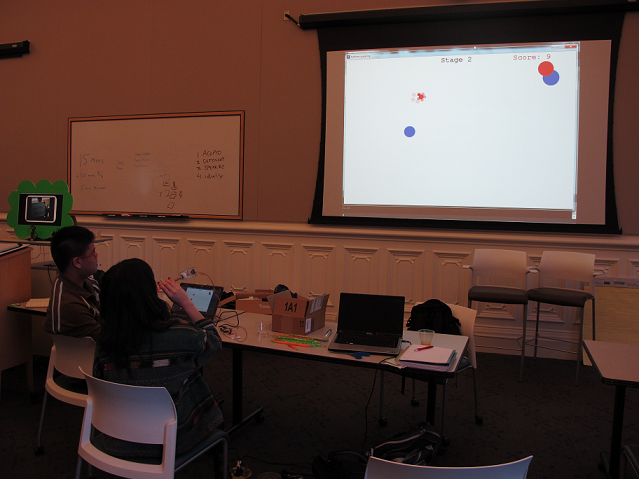
\includegraphics[width=\linewidth]{./figs/impl2.png}
  \caption{The participants trying out The Tangible Tube during a project showcase on December 7th 2011 at UC Berkeley campus.}
  \label{fig:impl2}
\end{figure}

The first thing that the testers do when trying out the \tube was figuring how to control the small pointer on the screen. Since there is feedback from the screen to show where the pointer is, the testers adapt to the system naturally and in no time successfully playing with \tube. The challenging part is when you have to match the color with the color of the balloon by rotating the tube. This is when the unique interaction with the system starts. The testers see that they cannot pop the balloon without matching the colors and start to rotate while blowing the tube.


\TODO
- Pictures \newline
- Describe the experience of the testers. \newline
- Evaluate how \tube is representative for games like balloon popping.
